\chapter{INTRODUCTION}\label{chap:INTRODUCTION}
\hspace{0.5in}This chapter describes the motivation, problem statement, scope of this project and objective of the Face Replacement System. It also describes the organization of this document.

\section{Motivation}

\hspace{0.5in}"One Picture is Worth Ten Thousand Words." This phrase can also mean that people love photography. When people go outside, travel in many places, they never forget the camera to take their photos. Nowadays, digital photography has become popular because of the cheaper cost and the convenience in taking and getting photos; photo film cameras are now obsolete.

People do not only collect their own photos, but they now love to share them with others, often through social networks, and this is called photo sharing. In order to share (or post) the photos on any social network, such as Windows Live, Facebook, MySpace, hi5, etc, users have to upload their photos on the Internet. Any internet user is able to search those photos by using a search engine in order to find the photos of someone they want to see.

However, sometimes photos are taken and accidentally include someone that the photographer did not want in that photo. The person who was accidentally shot in the photo may not even know. So, one important thing we should consider when photo sharing is privacy protection. One way to protect the privacy of the persons who were accidentally taken in the photo is to conceal their identity, especially their faces.

EveryScape.com is a web service which provides three-dimensional, photo-realistic experiences of cities \& towns, streets \& sidewalks, and building exteriors \& interiors. As shown in figure~\ref{fig:EveryScape}, this service provides the privacy protection which conceals the facial identity of people who are accidentally shot.

\begin{figure}[htb]
   \centering
   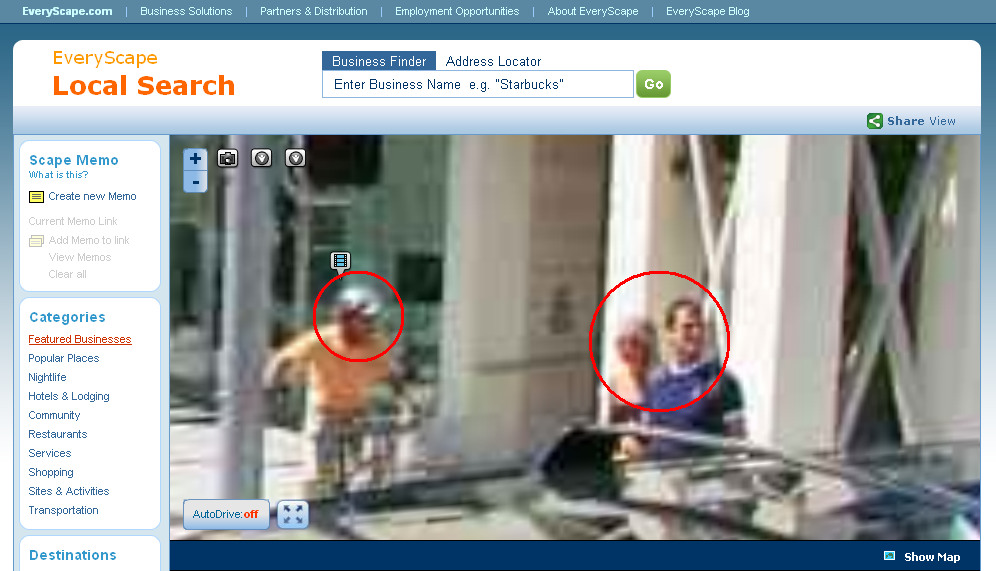
\includegraphics[width=12cm]{everyscape_privacy-protection_redcircle.png}
   \caption{EveryScape (http://www.everyscape.com)}
   \label{fig:EveryScape}
\end{figure}

People also love to have their photos to be satisfied, which means they should be good-looking in the photos they have taken. In group photos, the common situation occurs where people are not ready yet; eye closed, no smile, etc. So, these photos will be unsatisfactory. Not only these situations, but in others as well, people want to have fun with editing their photos to get them to look like a superstar, famous people, etc.

\begin{figure}[htb]
   \centering
   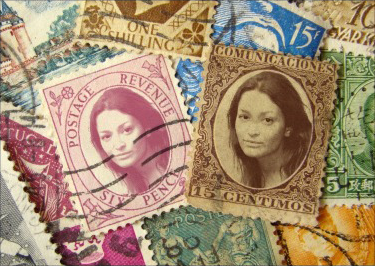
\includegraphics[width=8cm]{PhotoFunia_result.png}
   \caption{PhotoFunia (http://www.photofunia.com)}
   \label{fig:PhotoFunia}
\end{figure}

PhotoFunia.com is an online photo editing tool which provides the automatic creation of users' photos with many effects and montages.

People mostly consider how to look good such as to have a perfect body shape, to have nice skin especially, skin color, hair dressing, and even the dress; someone may try to wear the same clothes as famous people.
\begin{figure}[htb]
   \centering
   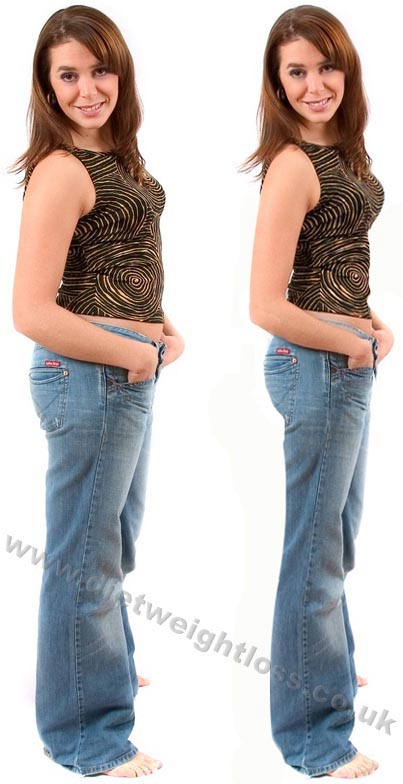
\includegraphics[width=5cm]{bodyshape_before-and-after.jpg}
   \caption{Before and After Manually Retouched Photo\\(http://www.dietweightloss.co.uk)}
   \label{fig:bodyshape}
\end{figure}

Often, there is one human part which people mostly consider, the face. The face can describe the expression, emotion, appearance, and beauty of humans. However, sometimes people are not satisfied with their photos; "It looks terrible", "Why so serious?", "I don't like this smile", etc. This is especially true in the event or the place that they will never be in again. They may not have a chance to take the photos like that again.

So, what people need is an image editing tool to edit their images to be more satisfied by improving unsatisfactory human appearance in their photos. There are many techniques using software tools that are now available to do image editing, but most people have no skill in image editing. Also, the cost of these tools are really expensive.

This project aims to help the users to create their satisfactory images by face replacement technique; to replace the imperfect face by a better face from another photo. It will be easy-to-use, and the result will come out as the final photo which users are really waiting for.


\section{Problem Statement}
\hspace{0.5in}As we had described in the previous section, privacy issues, difficulty to do try-on (superimpose someone's face on that of popular person), and unsatisfied appearance in the digital photographs are the problems that could be solved by digital image manipulation methods.

Most people want to edit their photos on their own but they have no skill in image editing. They will have to take much time to learn how to use these tools. Although they can do it well, they will take much time on doing it. In some image editing software such as Adobe Photoshop, they have to do it manually on each photo which will take much time or even some may give up on doing it because they lack art skill.

So, we need a system that will be easy to use and able to save time compared to the manually image editing software. And, a system that not only enables people to edit their photos in shorter time, but the result should also look real. The system should be able to combine one face to another head at the appropriate position \& pose, and the color \& lighting should be consistent.


\section{Objectives of the Project}
The purposes of this project are:
\begin{itemize}
\item To create an automatic face replacing tool. The tool is targeted for personal use, so it can be used by anyone, even the users with less image editing skill. The result should be created in reasonable time.
\item To create a face replacing tool which can produce a novel image that may never be taken again in the real events. It should look somewhat real.
\end{itemize}


\section{Scope of the Project}
\hspace{0.5in}This project aims to create an automatic tool to do image re-compositing on a coupling of a face and a head to get a new image. The system will need two input images. The first one is the source image of the face and  the other one is the image of the target head that users want to place the face on.

The approach of the system is to do alignment in 2D space. We are not going to create a 3D face model because it is hard to create one from only a single image and it may require too much user intervention. For some cases, some effort from users may be needed to help the system to do alignment.

We assume the pose of the face to be a frontal pose. The system will not support an out-of-plane pose because even the commercial face detector cannot correctly estimate the pose of the face from a single image. The system relies on the users to select the input images which have a similar pose, direction of light and shadow, color, and image resolution. For the extreme difference, the system might not be able to create the realistic result.

The result of the compositing of two images should be a picture that is blended seamlessly. The color will be changed from the source face image to the target head image.

This project is inspired by the research Face Swapping: Automatically Replacing Faces in Photographs by Dmitri Bitouk et al. In comparing Bitouk's Face Swapping and our system, it should be noted that, first, they swap any face in large image database to be out of context so, their system can automatically select the face arbitrarily, but our system takes images from users. Users can select the images from their personal photo collection. Second, they use a commercial face detector which has high quality face detection, but our system uses an open source face detector. Third, their system is designed to select only similar faces, whereas our system can take any face the users want. Fourth, their system uses simple feathering method to blend images, but our system needs to use better methods because our system cannot guarantee that the images are similar.


\section{Expected Benefits}
\hspace{0.5in}The system would enable the possibility to create new images that may never be taken again in the real events by any users. The system should be easy-to-use software which users do not need to have any image editing skills.

Furthermore, this system can be used as a privacy protector which would be useful when users would like to protect the privacy of people who accidentally appear in the photos by replacing the face identity before the photo is published.


\section{Organization of the Document}
This document consists of 6 chapters including:
\begin{enumerate}
\item Introduction - This chapter describes the motivation, problem statement, scope of this project and objectives of the Face Replacement System. It addresses some key questions. Why would we like to develop this system? What are the benefits of the system? It also describes the organization of this document.
\item Background - This chapter reviews the challenges which we have faced in order to develop the Face Replacement System. There are several methods with short descriptions which reference several related works.
\item Methodology - This chapter describes the chosen techniques in more detail, including mathematics formulae, and methods which are used in the system.
\item Implementation - This chapter shows the steps of work for the Face Replacement System and how we have developed the project.
\item Testing and Evaluation - This chapter shows experimental results of the testing and evaluation of using the Face Replacement System.
\item Conclusion - The last section of the document talks about benefits, problems and limitations and also future works of the Face Replacement System.
\end{enumerate} 